
\documentclass[crop,tikz]{standalone}

\usetikzlibrary{scopes}
\usetikzlibrary{arrows,shapes.gates.logic.US,shapes.gates.logic.IEC,calc}

\tikzstyle{gatestyle}=[draw = black,fill=lightgray,scale = 1.3,thick]

\begin{document}
   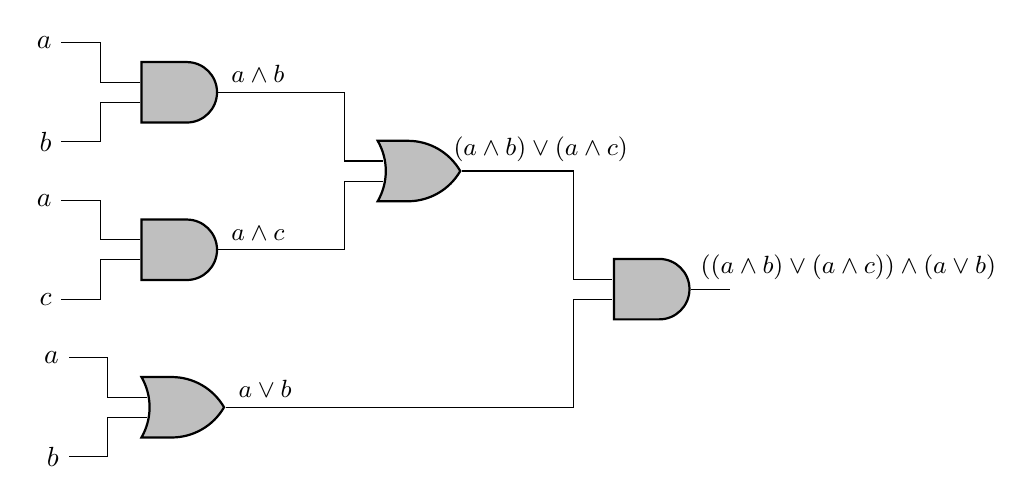
\begin{tikzpicture}

      % make these defs here so that I can change all after
      % note that you do not have to keep them consistent
      % I just defined this to make initial coding easier
      \def\xspace{3} % set the horizonal distance between gates
      \def\yspace{2} % set the vertical distance between gates
      \def\shift{0.5cm} % sets some spacing to draw connecting lines

      % Draw gates at nodes
      % define first col of gates
      \node[or gate US,gatestyle] at (0,0) (x1) {};
      \node[and gate US, gatestyle] at (0,\yspace) (x2) {};
      \node[and gate US, gatestyle] at (0,2*\yspace) (x3) {};
      % define second col of gates
      \node[or gate US, gatestyle] at ($0.5*(x2)+0.5*(x3)+(\xspace,0)$) (x4) {};\
      % define third col of gates
      \node[and gate US, gatestyle] at ($0.25*(x2)+0.25*(x3) + (2*\xspace,0)$) (x5) {};\

      % Draw all wires
      % Connect all gates internally
      \draw (x1.output) -| ([xshift = -\shift]x5.input 2) node (l1) {} --++(\shift,0);
      \draw (x4.output) -| ([xshift = -\shift]x5.input 1) --++(\shift,0);
      \draw (x2.output) -| ([xshift = -\shift]x4.input 2) --++(\shift,0);
      \draw (x3.output) -| ([xshift = -\shift]x4.input 1) --++(\shift,0);
      % draw end piece
      \draw (x5.output) --++ (\shift,0);
      % input positions (some work goes into making the text separated)
      % inputs 1
      \draw (x1.input 1) -|++ (-\shift,\shift) --++(-\shift,0) node[left,]{${a}$};
      \draw (x1.input 2) -|++ (-\shift,-\shift) --++(-\shift,0) node[left]{$b$};
      % inputs 2
      \draw (x2.input 1) -|++ (-\shift,\shift) --++(-\shift,0) node[left]{$a$};
      \draw (x2.input 2) -|++ (-\shift,-\shift) --++(-\shift,0) node[left]{$c$};
      % inputs 3`
      \draw (x3.input 1) -|++ (-\shift,\shift) --++(-\shift,0) node[left]{$a$};
      \draw (x3.input 2) -|++ (-\shift,-\shift) --++(-\shift,0) node[left]{$b$};

      % Insert labels
      \node[above] at ($(x3.output) + (\shift,0)$) (l1) {\small$a \land b$};
      \node[above] at ($(x2.output) + (\shift,0)$) (l1) {\small$a \land c$};
      \node[above] at ($(x1.output) + (\shift,0)$) (l1) {\small$a \lor b$};
      \node[above] at ($(x4.output) + (2*\shift,0)$) (l1) {\small$(a \land b)\lor (a\land c)$};
      \node[above] at ($(x5.output) + (4*\shift,0)$) (l1) {\small$((a \land b)\lor (a\land c))\land(a\lor b)$};

   \end{tikzpicture}

\end{document}